\section{Mechanism: Offline Work and Delayed Synchronization}
\label{sec:mechanism}

\subsection{Main backlog measure}
\label{sec:backlog}

A fall in public GitHub events does not necessarily imply an equal fall in code creation. Git is decentralized: developers may continue editing files and creating commits locally, then push them only after connectivity returns. The commit-level analysis directly tests for this pattern.

In the strict sample, 2,932 commits are authored during July 18--23. Of these, 829 first appear in a public push on or after July 24. The resulting author-time backlog share is 28.27 percent (\cref{tab:mechanism}). Replacing the author timestamp with the committer timestamp produces a nearly identical 27.16 percent backlog share (790 of 2,909 commits). The agreement between the two metadata clocks is useful because neither timestamp is a perfect external record of when coding occurred. Both timestamps are Git metadata generated by the author's local client or the hosting platform at commit time, not an externally verified record of the exact physical moment the code was written; the mechanism evidence is therefore consistent with offline or local work followed by delayed synchronization, but it does not directly observe the underlying production process.

Long publication delays become dramatically more common during the shutdown. Among shutdown-authored commits, 29.71 percent have an author-to-push delay above 24 hours, 25.38 percent above 48 hours, and 22.75 percent above 72 hours. In six overlapping pre-shutdown placebo windows, the corresponding averages are approximately 1.10 percent, 0.72 percent, and 0.46 percent (\cref{tab:mech_placebos}). Because commit metadata were queried for only a daily sample of commits pushed before July 18 but for all commits pushed from July 18 onward, the placebo rates use inverse-probability weights, while shutdown-authored commits, all pushed on or after July 18, receive weight one. The real shutdown is therefore far outside the normal pre-period delay distribution.

% Generated by analysis/tables/make_all_tables.py -- do not edit by hand.
\begin{table}[htbp]
\centering
\footnotesize
\caption{Commit-time mechanism}
\label{tab:mechanism}
\begin{threeparttable}
\begin{tabular}{lrrrrrrr}
\toprule
Timestamp & $N$ during & Pushed & Backlog & $>$24h & $>$48h & $>$72h & Mean \\
 & shutdown & Jul 24+ & share & & & & delay (h) \\
\midrule
\texttt{authoredDate} & 2,932 & 829 & 28.27\% & 29.71\% & 25.38\% & 22.75\% & 40.94 \\
\texttt{committedDate} & 2,909 & 790 & 27.16\% & 28.60\% & 24.27\% & 21.73\% & 37.47 \\
\bottomrule
\end{tabular}
\begin{tablenotes}[flushleft]
\footnotesize\raggedright
\item \textit{Notes:} Strict sample requires author login = PushEvent actor, a non-missing timestamp, and a nonnegative delay. The backlog share is conditional on commits observed in the mechanism sample, not a share of all software production in Bangladesh. \texttt{authoredDate} and \texttt{committedDate} are Git metadata, not externally verified measurements of when code was written.
\end{tablenotes}
\end{threeparttable}
\end{table}


\subsection{Timing and concentration of delayed pushes}
\label{sec:timing}

The delayed commits are released quickly once connectivity begins to return (\cref{fig:mechanism}). Of the 829 author-time backlog commits, 354 (42.7 percent) appear on July 24 and 544 (65.6 percent) by July 25. By July 27, 81.1 percent have appeared; by July 31, 92.0 percent have appeared. This temporal concentration immediately after restoration is consistent with a synchronization backlog rather than ordinary long-lived branches or sporadic publication.

\begin{figure}[htbp]
\centering
\caption{Release timing of commits with shutdown-period Git author timestamps}
\label{fig:mechanism}
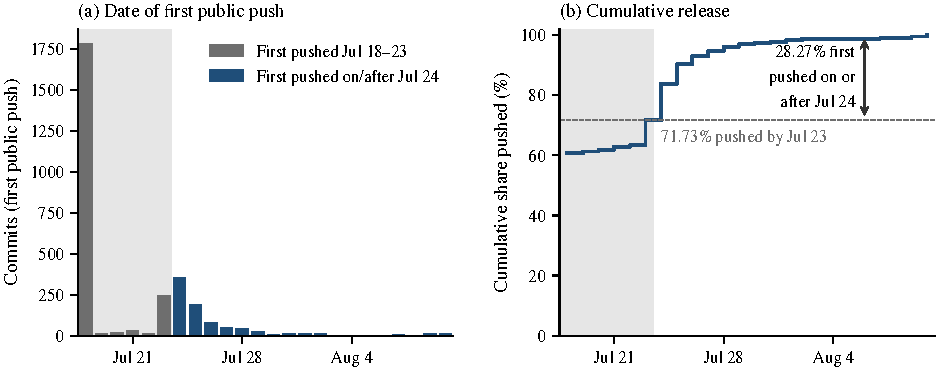
\includegraphics[width=\textwidth]{fig4_mechanism_release.pdf}
\fignote{Strict sample: commits whose GitHub-linked author equals the Bangladeshi pusher, with a non-missing author timestamp and nonnegative author-to-push delay; the cohort is the 2,932 commits authored July 18--23 (UTC). Panel (a): date of first public push; panel (b): cumulative share pushed. 829 commits (28.27\%) first appear on or after July 24; pushes are observed through August 10. Git \texttt{authoredDate} and \texttt{committedDate} are metadata, not verified measurements of when code was written; the pattern is consistent with local work followed by delayed synchronization. The share refers only to this strict sample, not to all software production in Bangladesh. Source: Author's calculations using GH Archive and GitHub commit metadata.}
\end{figure}

The backlog is not generated by only a handful of unusually active users (\cref{tab:concentration}). The 2,932 shutdown-authored commits come from 835 users and 977 repositories. Two hundred twenty-two users (26.6 percent) and 246 repositories (25.2 percent) contribute at least one backlog commit. The largest user accounts for 2.77 percent of backlog commits, the top five users for 12.06 percent, and the top ten for 21.47 percent. Dropping the twenty users with the most backlog still leaves a 20.37 percent backlog share.

Backlog is, however, more common in larger pushes (\cref{tab:push_size}). Restricting to pushes with at most 10 commits lowers the backlog share to 21.0 percent; at most 5 commits, 14.4 percent; at most 2 commits, 7.8 percent; and single-commit pushes, 3.3 percent. This pattern is economically meaningful rather than merely inconvenient: if developers accumulate local commits while offline and synchronize later, restoration should produce larger-than-normal push batches. At the same time, it means that the 28.3 percent headline mechanism estimate should not be interpreted as applying uniformly to every kind of push.
